\section{Описание}

Для выведения графика я написал небольшой скрипт, который из специально заготовленного файла считывает данные о токенах, а затем выводит графики.

Для закона Ципфа я использовал следующую формулу:

$$ r = \frac{k}{f} $$
где $k$ - константа, $r$ - ранг токена, $f$ - частота слова

В качестве константы я взял максимальное значение частоты из всех частот слов.

Помимо этого попробовал приложить ещё и формулу Мандельброта:

$$ P * (t + \rho)^{-B} $$ 
где $P$, $B$, $\rho$ - константы.

Подбором взял $P = 10^{7.2}$, $\rho = 1$, $B = 1.05$, так они были наиболее близки к графику частот.

\pagebreak
По итогу вышла следующая ситуация (по оси X - ранг, по оси Y - частота):

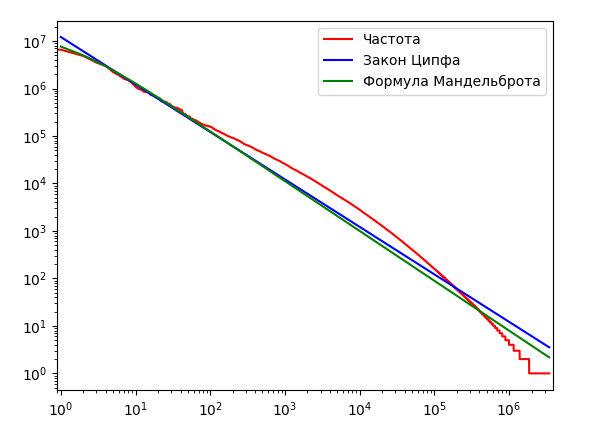
\includegraphics{1.png}

Ключевое замечание - частота слов довольно сильно откланяется закона Ципфа. Можно попробовать поставить график несколько выше, увеличив значение константы, но тогда будет заметно ещё большее отклонение в местах с малым и высоким рангом.

Касательно Мандельброта - я постарался подобрать $\rho$ и $P$ таким образом, чтобы график совпадал с графиком частот при малом ранге, но при средних и высоких значениях ранга разница всё ещё ощутимая. Попытки слегка измений наклона графика за счёт константы $B$ не очень увенчались успехом.

В целом такой изгиб в частотах говорит, как мне кажется, что те дампы Википедии, что я взял, содержат в себе такой набор слов, который характерен только лишь этим дампам. Т.е. если взять весь дамп Википедии, а не только её часть, скорее всего этот изгиб станет гораздо менее явным или вовсе пропадёт.

Касательно участка с малой частотой - там заметны характерные горизонтальные линии. По сути это большое количество различных слов, которые попадались крайне редко. Среди них также много различного мусора, который не удалось выловить текущим парсером, так что если бы реализация парсера учитывала больше вариантов, то горизонтальные линии были бы короче.

\lstset{extendedchars=\true}
\section{Исходный код}

Скрипт для вывода графиков:
\begin{lstlisting}[language=Python]
from numpy import *
import matplotlib.pyplot as plt

counter = dict()
tmp = 0
with open("total.data", "r") as file:
    for line in file:
        str = line.split(" ")
        if len(str) > 1:
            counter.update({str[0]: int(str[1])})

values = sorted(counter.values(), reverse=True)
len_values = len(values)
ids = [i for i in range(len_values)]

t = linspace(1, len_values, len_values)
a = values[0] / t
b = power(10, 7.2) * power(t + 1, -1.05)

fig = plt.figure()
ex = fig.add_subplot(111)
ex.plot(ids, list(values), 'r', label="Частота")
ex.plot(t, a, 'b', label="Закон Ципфа")
ex.plot(t, b, 'g', label="Формула Мандельброта")
ex.set_yscale("log")
ex.set_xscale("log")
ex.legend()
plt.show()
\end{lstlisting}